\chapter{Tooling}

\section{Java Enterprise Edition}
Java Applikationen, welche auf Java EE basieren, werden in einem Applikationsserver deployt. Dieser stellt verschiedene Laufzeitumgebungen sogenannte Container zur Verfügung. Diese Container sind Zusammenstellungen aus diversen Frameworks, welche immer einer Java Spezifikation (JSR) folgen. Beispielsweise ist das Java Persistence API ist im JSR 317 spezifiziert. Die Komplexität wird durch das Verwenden der vielen Frameworks erhöht, jedoch muss damit nicht jedes mal das Rad neu erfunden werden.

\section{Applikations-Server}
Im Java EE 6-Standard (JSR 316) sind zwei unterschiedliche Profile für Applikation-Server definiert:

\begin{description}
	\item[Full Profile:] Beinhaltet all Spezifikationen zu Java EE 6.
	\item[Web Profile:] Beinhaltet eine Untermenge aller Spezifikationen von Java EE 6.
\end{description}

Das Web-Profile soll eine \emph{lightweight} Variante eines Java-EE Applikations-Server darstellen. Dabei werden tendenziell auf komplexere Services verzichtet, welche in grossen Infrastrukturen zum Einsatz kommen (wie JMS). Websphere, GlassFish und WildFly implementieren das Full Profile. Das Web Profile wird von WebSphere Liberty und von Apache TomEE angeboten.

Die Hersteller bieten nebst den genannten Profilen auch noch eigene Profile an. Diese unterscheiden sich im Umfang der eingebauten Spezifikationen. Der Apache TomEE deckt das gesamte Web Profile ab und der Apache Tomcat nur eine Untermenge daraus. Man kann gut und gerne auch eigene Technologien selbst einbinden - klappt gut, falls mal etwas in einem konkreten App-Server fehlt.

Beispielsweise hat der Apache Tomcat  standardmässig JPA nicht dabei (muss selber mitdeployt werden). App-Server mit dem Web-Profile, hätten es bereits zur Verfügung.

\section{Container}
\begin{itemize}
	\item Laufzeitumgebung im Applikationsserver
	\item Applikation wird in einem Container deployt
	\item Stellt der Applikation Services zur Verfügung (Bsp. Datenbankzugriff)
\end{itemize}

\begin{figure}[h!]
\centering
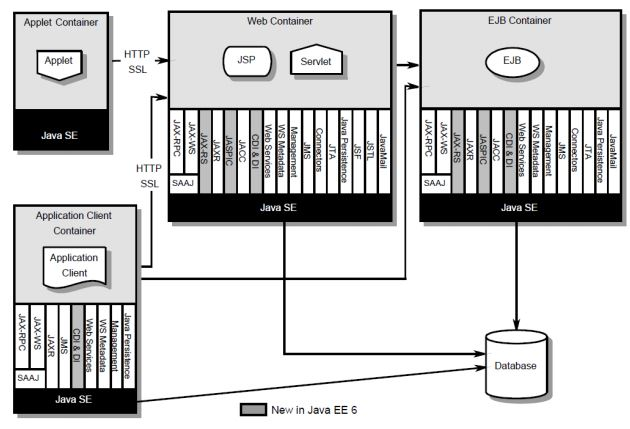
\includegraphics[width=0.7\linewidth]{fig/tooling-container}
\caption{Tooling - Container}
\label{fig:tooling-container}
\end{figure}

\subsubsection{Container-Typen}
\begin{itemize}
	\item Applet-Container
	\item Application Client-Contaier
	\item Web-Container (synonym: Servlet-Container) (Kann mit HTTP umgehen.)
	\item EJB-Container.
\end{itemize}

\subsubsection{Anwendungs-Komponenten}
\begin{itemize}
	\item Applets (GUI-Anwendungen, die normalerweise im Browser ausgeführt werden; heutzutage eher veraltet)
	\item Application Clients (eigenständige GUI-Applikationen auf den Client-Rechnern, z.B. in Swing, JavaFX oder ähnlichen Technologien realisiert)
	\item JSP und Servlet (stehen für eine ganze Familie von Web-Komponenten)
	\item EJB (Geschäftslogik in einer transaktionsunterstützen Umgebung)
\end{itemize}


\section{DB2}
DB2 ist von IBM und im Unternehmensumfeld stark verbreitet. Auf einem Server können mehrere DB2 Instanzen betrieben werden. Jede Instanz kann mehrere Datenbanken haben. Nun folgen die Schemas und erst dann die Tabellen. Wir haben im ENAPP-Modul eine Instanz betrieben, welche die Datenbank ENAPP beinhaltet und haben dann Schemas wie SBBRSS, EATME oder eben WEBSHOP erzeugt. (\emph{“In MySQL, physically, a schema is synonymous with a database}).

\begin{lstlisting}
student@linux-wm6v:~> su - db2inst
Password:

db2inst@linux-wm6v:~> db2
...

db2 => CONNECT TO ENAPP
Database Connection Information
Database server = DB2/LINUXX8664 10.5.5
SQL authorization ID = DB2INST
Local database alias = ENAPP

db2 => SELECT * FROM SBBRSS.ITEMS
... 4 record(s) selected.

db2 => QUIT
DB20000I The QUIT command completed successfully.

db2inst@linux-wm6v:~> exit
logout

student@linux-wm6v:~>
\end{lstlisting}

Wenn mit JPA auf ein Schema zugegriffen wird, reichen logischerweise die Standard-Verbindungsdaten nicht aus. Darum muss hier beispielsweise ein \verb|orm.xml| mit folgendem Inhalt zusätzlich definiert werden:

\begin{lstlisting}
...
<persistence-unit-metadata>
	<persistence-unit-defaults>
		<schema>SBBRSS</schema>
	</persistence-unit-defaults>
</persistence-unit-metadata>
...
\end{lstlisting}

\section{Facetten}
Damit bei einer Applikation nicht immer einfach alles mit deployt wird, können Erweiterungen über Facetten definiert werden. In einem Web Projekt, welche direkt über JPA auf die DB zugreift, kann die JPA Facette hinzugefügt werden. \emph{Facets define characteristics and requirements for Java EE projects and are used as part of the runtime configuration.}




\section{Projektstruktur von Java EE Projekte}

\begin{description}
	\item[EatMeMine:] Das ist das Projekt, in das die einzelnen Teilprojekte (EJB, Web, Client) später
	zusammengepackt werden und als Ganzes auf den Server deployen wird.
	
	\item[EatMeMineEJB:] „EJB“ steht für Enterprise JavaBeans. Dieses Projekt beinhaltet den Teil der
	Applikation, der für die Geschäftslogik verantwortlich ist. Sie sind das Prunkstück von Java EE, da
	sie Services wie Transaktionen, Security oder Job scheduling bieten.
	
	\item[EatMeMineWeb:] Web-Projekt mit Servlets, Managed-Beans, JSF und allem anderen Web-Geschmäus (HTML, CSS, JS).
	
	\item[EatMeMineClient:] Dieser ist dazu da, ein reines standalone Java-Programm mit unserer	Geschäftslogik – sprich unserem EJB-Projekt – plaudern zu lassen. Dies kann beispielsweise eine Konsolen- oder Swing-Applikation sein.
\end{description}

Der Unterschied zwischen einem (Tomcat-)Webprojekt und einer (WebSphere-)Enterprise Applikation liegt im Wesentlichen beim EJB-Projekt.

\subsection{Archive}

\begin{itemize}
	\item „Normale“ standalone Java-Programme (hier z.B. der „EatMeMineClient“) in JARs gepackt und anschliessend ausgeführt.
	\item Die Archivart für EJB-Projekte („EatMeMineEJB“) ist ebenfalls JAR.
	\item Für Webprojekte („EatMeMineWeb“) heisst die Archivart WAR (web archive).
	\item Für Enterprise-Applikationen („EatMeMine“) heisst die Archivart EAR (enterprise archive).
	\item Ein EAR beinhaltet ein oder mehrere WAR- und EJB-Archive bzw. JAR-Archive.
	\item Alle diese Archivarten sind technisch nichts anderes als ZIP-Archive, in die man dementsprechend mit jedem Unzipper reinschauen kann.
\end{itemize}
Nebst diesen Projekten legen wir noch ein common-Projekt mit Interfaces an.

\section{Java EE-Architektur: MVC Model 2}

\begin{figure}[h!]
\centering
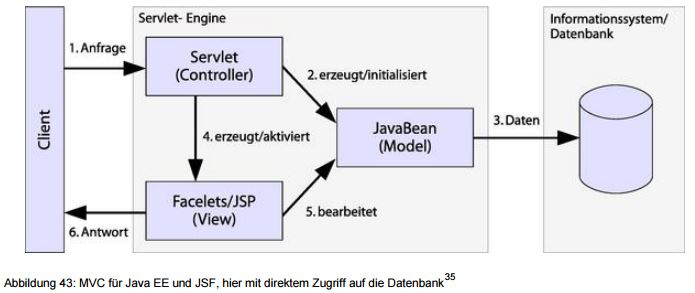
\includegraphics[width=0.7\linewidth]{fig/tooling-mvc-im-view-layer}
\caption{MVC im View Layer mit Hilfe von JSF umgesetzt}
\label{fig:tooling-mvc-im-view-layer}
\end{figure}
\begin{itemize}
	\item Das Faces Servlet ist der Controller. Du kennst ja inzwischen die Funktion eines Servlets, und
	lucky us: wir müssen für die Verwendung von JSF als View-Technologie, die wir ab Kapitel 5
	verwenden werden, kein eigenes Servlet schreiben. Das Faces Servlet nimmt die Anfragen
	entgegen und interagiert mit der View und ihrem Status.
	\item Managed Beans werden von der Programmiererin erstellt und enthalten den Java-Code für den
	View-Layer, sind also quasi das „Model der View“. Siehe den Hinweis zu Managed Beans im
	Anschluss. Sie sind für die Verbindung zur Geschäftslogik zuständig.
	\item  Die View besteht aus xhtml-Seiten und Facelets. Das ist mit zusätzlichen Tags erweitertes
	(X)HTML, in welches dynamische Inhalte über den Aufruf von Methoden an den Managed Beans
	eingebunden werden.
	\item  Die Geschäftslogik ist im EJB-Projekt gekapselt. Somit ist auch klar, dass das gesamte WebProjekt
	keine Geschäftslogik enthält! Und somit wird die Planung ganz wichtig.
\end{itemize}

\emph{Der Begriff Managed Bean ist nicht eindeutig. Mit der Annotation @ManagedBean wird im Code eine Bean beschrieben, die von einer xhtml-Seite aus erreichbar ist. Wird ein Web-Projekt ohne	EJB-Projekt deployt (so wie in der Tomcat-Übung in Kapitel 3), ist die Geschäftslogik, bzw. ein Teil davon, ebenfalls in der Managed Bean enthalten. In einer vollständigen Enterprise-Applikation andererseits ist die Geschäftslogik im EJB-Projekt gekapselt. Somit gilt: Für eine Web-Applikation gehören die Managed Beans zum Model, in einer Enterprise Applikation nur zur View.}

\begin{figure}[h!]
\centering
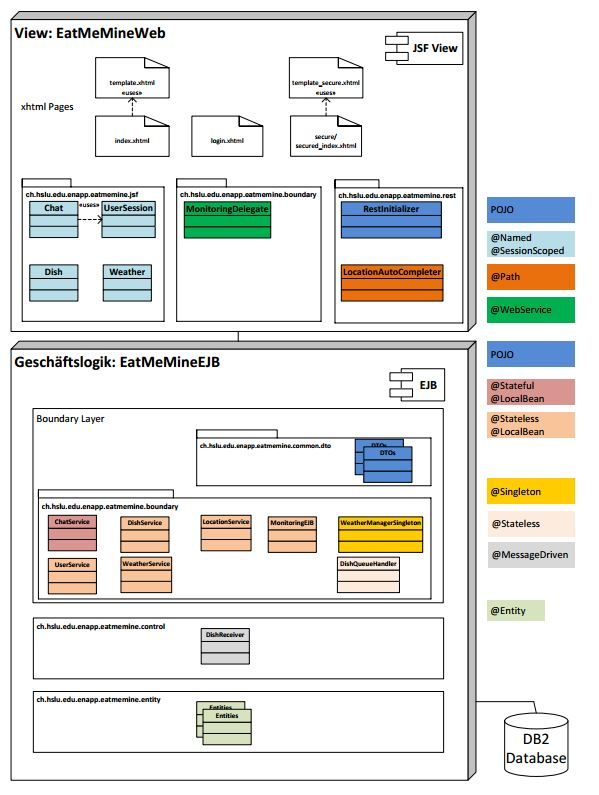
\includegraphics[width=0.7\linewidth]{fig/tooling-architektur-eatmemine}
\caption{Architektur EatMe Mine}
\label{fig:tooling-architektur-eatmemine}
\end{figure}


\section{EJB}
EJBs sind container managed und werden immer über @Inject bzw. @Ejb injiziert. Also nie mit new-Erzeugen! Man sollte falls möglich @Inject verwenden. Der wesentliche Unterschied zwischen @Inject und @EJB ist, dass mit @Inject Instanzen vieler verschiedener Klassen-Typen (sogar POJOs) injiziert werden können, mit @EJB hingegen wirklich nur EJBs. Dass es sich bei einer Klasse um eine EJB handelt, erkennst du an der Annotation @Stateful oder @Stateless. Andererseits ist es manchmal notwendig, Attribute bei der Annotation anzugeben, was wiederum bei @Inject nicht möglich ist. An dieser Stelle wird dann nicht das echte EJB injiziert sondern ein Proxy, welche sich dann aufen Scope (SessionScope, RequestScope, ...) bezieht.

\subsection{EJB-Typen}

\begin{description}
	\item[@Local] Die EJB, die ein solches Interface implementiert, kann von allen Modulen (z.B. einem WAR) innerhalb derselben JVM verwendet werden. „Innerhalb derselben JVM“ bedeutet also beispielsweise	von allen Anwendungen innerhalb des Applikationsservers. (@Inject/@EJB)
		
	\item[@Remote] EJBs die ein solches Interface implementieren, können auch von Modulen ausserhalb der JVM, in der die Applikation läuft, erreicht werden. Dieser Interface-Typ wird vor allem von Application-Clients	genutzt, welche als native Java-Applikation an ein EJB-Modul andocken. Genau eine solche Konsolenapplikation werden wir am	Anfang zum Testen unserer Geschäftslogik verwenden. (@EJB)
	
	\item[no Interface / @LocalBean] „No interface“ (also keine Annotation) und die Annotation	@LocalBean meinen dasselbe. Solche EJBs sind nur für die Module innerhalb ihres EARs sichtbar.	(@Inject/@EJB)
\end{description}
 
Mit der Festlegung des Typs einer Session Bean legen wir fest, ob eine sie ihren Status über eine ClientSession hinweg behalten soll (@Stateful) oder eben nicht (@Stateless). Der UserService beispielsweise
soll lediglich den User in der Datenbank suchen und falls er existiert zurückmelden, ob das Passwort stimmt. Natürlich sollen auch neue User eingetragen werden können. Um diesen Job zu erledigen muss
sich die Bean aber keinen Status merken, deshalb erzeugen wir sie @Stateless. Beim ChatService sieht dies anders aus. Hier wollen wir uns merken, welcher User (also welcher angemeldete User, also welche Session) gerade mit der Bean kommuniziert. Deshalb ist sie stateful. Es gibt noch eine weitere Art von Session Bean, @Singleton.

\section{Application Client}
Wenn wir nun aus einer Java SE Umgebung auf die EJB zugreifen wollen müssen wir wie folgt vorgehen:
\begin{itemize}
	\item Beans müssen mit @Remote annotiert sein - da wir aus einer anderen JVM auf die Beans zugreifen wollen.
	\item Interfaces sollten daher auch in einem common-Projekt ausgelagert sein, damit es sowohl vom Bean-Projekt wie auch vom Client-Projekt verwendet werden kann.
	\item Im Client-Projekt müssen wir beim Injecten den Lookup angeben \\ \verb|@EJB(lookup = "ch.hslu.edu.enapp.eatmemine.common.ChatServiceRemote")|.
	\item Das Client Projekt wird innerhalb des EAR deployt und kann auf der Konsole wie folgt aufgerufen werden:
	\verb|/opt/IBM/WebSphere/AppServer/profiles/AppSrv01/bin/launchClient.sh|\\
	\verb|/home/student/workspace_WAS/EatMeMineProject/EatMeMineExports/EatMeMine.ear|\\
	\verb|-CCproviderURL=iiop://localhost:2809/|
\end{itemize}

Ich weiss auch nicht genau was das bringen soll. So kann man einfach Konsolen-Applikationen erstellen, aber der Nutzen sehe ich nicht.

\section{Java Server Faces}
Früher hat man JSP (Java Server Pages) verwendet. JSF hat diese Technologie abgelöst. In JSF wird der Webteil in .xhtml abgehandelt. Es enthält extended HTML Tags. 

\begin{lstlisting}
<html xmlns="http://www.w3.org/1999/xhtml"
	xmlns:h="http://java.sun.com/jsf/html"
	xmlns:ui="http://java.sun.com/jsf/facelets">

<h:head>
	<title>index</title>
	<meta http-equiv="Content-Type" content="text/html; charset=UTF-8" />
</h:head>
<h:body>
	<p>Das ist ein Test.</p>
</h:body>
\end{lstlisting}

Es müssen Servlet-Mappings angegeben werden. Es werden nur xhtml-Dateien mit JSF verarbeitet, welche dem folgenden Pattern entsprechen:

\begin{lstlisting}
<servlet-mapping>
	<servlet-name>Faces Servlet</servlet-name>
	<url-pattern>*.xhtml</url-pattern>
</servlet-mapping>

<!-- Mit dieser Konfig sehen wir mehr Fehlemeldung -->
<context-param>
	<param-name>javax.faces.PROJECT_STAGE</param-name>
	<param-value>Development</param-value>
</context-param>
\end{lstlisting}

Um nun mit Java-Code zu interagieren, rufen wir aus den .xhtml Dateien sogenannte Managed Beans auf:

\begin{lstlisting}
<h:body>
	<h:outputText value="#{chat.testMe}" />
</h:body>

@Named
@SessionScoped
public class Chat implements Serializable {
	private static final long serialVersionUID = 1L;
	private final String testMe = "Hello World";
	public String getTestMe() {
		return testMe;
	}
}
\end{lstlisting}

Wenn mit Dependency Injection in diesem Umfeld gearbeitet wird, sollte man achten, dass man nur ein Framework verwendet (javax.enterprise.context.*).

\section{WebSphere}
Der WebSphere hat eine Admin-Shell-Konsole (/home/student/IBM/WebSphere/AppServer/profiles/AppSrv01/bin/wsadmin.sh). Zudem ein webbasierte \emph{INtegrated Solution Console}  (Admin-Konsole, Web-Konsole) unter https://localhost:9043/ibm/console. Zudem gibt es den Universal Test Client. Dies ist auch eine Web-Oberfläche wobei man alle installierten Beans sehen kann und die Methoden direkt aufrufen. Beispielsweise müssen die gesamten Verbindungsdaten zur von App-Server zur DB professionel auf dem App-Server konfiguriert werden. Die Applikation soll nicht die Verbindungsdaten mitgeben, denn der Entwickler weiss zu diesem Zeitpunkt ja gar nicht, wohin die Ware deployt wird.

\subsection{Konfiguration DB-Verbindung}
\begin{enumerate}
	\item Anlegen eines JDBC Providers (für DB2)
	\item Anlegen einer Data Source, welche über den angelegten JDBC Provider kommuniziert. Hier werden DB Name, Server Name und Port definiert. Das Schema muss über \emph{custom properties} separat definiert werden (currentSchema). Zudem muss auch der JNDI Namen eingetragen werden. Die Applikation kann sich auf diesen beziehen und so zur DataSource kommen.
	\item Nun müssen noch die Credentials angelegt werden. Also JAAS - J2C authentication data. Darin wird ein Alias definiert sowie Benutzername und Passwort. Dieser Alias wird nun mit der DataSource gekoppelt.
	\item Im \verb|persistence.xml| kann nun einfach \verb|<jta-data-source>jdbc/sbbrss</jta-data-source| definiert werden. Der ganze andere Verbindungs-Kram fällt weg.
\end{enumerate}

\subsection{Konfiguration JMS}
\begin{enumerate}
	\item Busname erzeugen
	\item Destination definieren
	\item Queue connection factoriy definieren (In den JDNI hängen)
	\item Queue selbst definieren (In den JDNI hängen)
\end{enumerate}